\documentclass[../Cryptography.tex]{subfiles}

\begin{document}
\chapter{Public-key cryptography}
\section{Going public}
\subsection{Symmetric crypto vs public-key crypto}
Symmetric cryptography is the oldest kind of cryptography. Indeed, the idea of having a public key is quite disturbing at first glance. Just a quick reminder, here is how we settle a supposed secure way of communication between Ali and Bachar using public-key crypto.

\begin{enumerate}
    \item Ali and Bachar both generate a key-pair : they keep one private for each, and they publish the other, making it public, so anyone has access to Ali and Bachar's public key.
    \item If Bachar wants to send a message to Ali, he \textbf{encrypts with Ali's public key} and sends him
    \item Ali receives messages that are encrypted using his public key. He decrypts them using his private key.
\end{enumerate}

That's the kind of communication we have for public-key crypto. Symmetric crypto was based on the idea of having \textbf{only one key}, kept secret, between A and B. 
\subsection{Why going public ?}
There are many problems to symmetric crypto :
\begin{itemize}
    \item Key distribution problem : the key must be established between Ali and Bachar. How do they do ? The communication link between them is not secure.
    \item Number of keys : if there are $n$ users, there are $n(n-1)/2$ keys. That's a lot ! 4 million keys for 2000 people.
    \item No protection against cheating : as Ali has the same secret key as Bachar, he can create a message from scratch and claim that Bachar created it.
\end{itemize}

In addition to all this, let me talk a little bit, because you guys talk too much, 
\includegraphics[width=2cm]{images/khabib.png}. Symmetric crypto algorithms are meant to avoid any compact mathematical description. That is easy shit. Asymmetric crypto is \textbf{built on one-way number-theoric functions so there is no bullshitting in their security}, you get me ?

\subsection{Actually going public}
When going public, we are immediately subject to a particular kind of attack : the \textbf{Man-In-the-Middle attack} (MIM\footnote{Pas MYM, mécréant.}). In public-key crypto, a crucial part is the exchange of keys : Ali gives his public key to Bachar, so that Bachar can send him messages, and inversely. But there can be an outsider Omar that acts as follows : 
\begin{itemize}
    \item He captures Ali's public key $k_A$ before Bachar gets it
    \item He sends to Bachar a false public key, being his own, $k_O$
    \item Bachar sends his public key to Ali but it gets intercepted by Omar, that gives to Ali his $k_O$ instead.
    \item Ali thinks he is receiving messages from Bachar, and inversely, but it is actually the no-life Omar that is intercepting everything and manipulating the conversation. \\
\end{itemize}
To avoid this, we make use of \textbf{certificates}, objects that bind a public key to an identity. A public key certificate is an object that contains :
\begin{itemize}
    \item The public key
    \item Information allowing to identify its owner, such as the name, the ID, IP, etc.
    \item A digital signature on the key and the information : this is signed by a \textbf{certification authority}.
\end{itemize}

Thanks to this, at the end, Omar can not generate a fake certificate using his key and Ali's information because the signature will be different than Ali's public key certificate, and Bachar will notice that. The certification authority must of course be trustworthy.  We can also build hierarchies between CAs as seen below.\\

\begin{center}
    \includegraphics[width=0.45\linewidth, page=9]{Slides/4-Public.pdf}
    \includegraphics[width=0.45\linewidth, page=10]{Slides/4-Public.pdf}
\end{center}

Let us recall that we solve only a part of the problem, because Omar can still intercept the communication between Ali and the CA ! Hence, we must have a \textbf{secure authenticated channel with the CA}. \\

\subsection{Hybric encryption}
Note that in practice, we use \textbf{hybrid encryption} to improve both efficiency and bandwith (avoid transmitting a lot of data). 
\begin{center}
    \includegraphics[width=0.8\linewidth, page=13]{Slides/4-Public.pdf}
\end{center}


There are many ways of doing public-key crypto, based on different mathematical problems. There is \textbf{large integer factorization} ($\rightarrow$ RSA), \textbf{discrete logarithm problem} ($\rightarrow$ ElGamal DSA, and DH), and \textbf{elliptic curves} ($\rightarrow$ ECDSA)
\section{RSA : a factorization problem}
RSA is mainly about key generation. It is an interessant way of generating keys but is subject to a lot of attacks. 
\subsection{Key generation}
The key generation relies on the fact that factorizing large integers is complicated. Hence, it is based on two prime numbers $p$ and $q$, kept private but \textbf{their product $n$ is kept public}, as part of the public key. \\

The other part of the public key is an exponent that will come in play when encrypting. We note it $e$. It is public, and satisfies $$3 \leq e \leq (p-1)(q-1) - 3 \qquad \mathrm{gcd}(e, (p-1)(q-1)) = 1 \; .$$
Often, one chooses $e$ and then generates the primes. \\

The private key is the inverse of $e$ modulo $(p-1)(q-1)$. 

\begin{center}
    \includegraphics[width=0.6\linewidth, page=35]{Slides/4-Public.pdf}
\end{center}

\subsection{RSA textbook encryption}
Here is an encryption scheme that stinks a lot : we elevate the message to the power of $e$ to get the ciphertext. To decrypt the ciphertext, we elevate it to the power of $d$, as $e$ is the inverse of $d$.
\subsection{RSA textbook signature}
It is basically similar, but here we are \textbf{signing} a message with the private key, so $s = m^d \mod{n}$. Again, to check the signature, we can elevate $s$ to the power of $e$ to verify if we indeed get the message back (valid signature) or not.

\begin{center}
    \includegraphics[width=0.45\linewidth, page=37]{Slides/4-Public.pdf}
    \includegraphics[width=0.45\linewidth, page=38]{Slides/4-Public.pdf}
\end{center}

\subsection{Attacks on RSA}
RSA is subject to many attacks, one of the easiest ones being the \textbf{short message attack}, when we know that $e$ is small. We can send short messages so the modular reduction by $n$ does nothing in the encryption. So we can find back $m$ by taking the $e$-th root of $c = m^e$. One just has to try the different $c$s.

\subsection{Powering RSA}
\subsubsection{RSA-OAEP : optimal asymmetric encryption padding}
Padding is really interesting. We here add padding to the original message, and randomness to the pre-processing of the message before encryption. Encryption is done as always, exponentiating by $e$, moduling by $n$, but the input is a new one : the message after pre-processing. 

\begin{center}
    \includegraphics[width=0.8\linewidth, page=47]{Slides/4-Public.pdf}
\end{center}
This helps with the short message attack, makes the scheme probabilistic, and introduces diffusion. In addition, it is shown to be IND-CCA secure. Wow !

\subsubsection{RSA-KEM : Key Encapsulation Method}
Here, we present a method to do \textbf{hybrid encryption} using RSA. It is not an encryption scheme that we present ! Remember that in hybrid encryption, Ali somehow chooses the symmetric key and sends it to Bachar in an encrypted way. Here we will have something different : 
\begin{itemize}
    \item Ali chooses a random string $m$ of size $n$, where $n$ is part of his RSA public key.
    \item He hashes $m$ : gives $k = \mathrm{hash}(m)$ which will be the secret key
    \item Ali encrypts $c = m ^e \mod{n}$, and sends $c$ to Bachar 
\end{itemize}

To decrypt (actually, \textit{decapsulate}), Bachar does the following :
\begin{itemize}
    \item Recovers $m = c^\rouge{d} \mod{n}$
    \item Computes $k = \mathrm{hash}(m)$
\end{itemize}
We thus see that the key $k$ is encapsulated in $m$, himself encrypted by RSA textbook encryption.

\subsection{Computational analysis of RSA}
Encryption in RSA consists in two operations : exponentiating for encrypting, exponentiating for decrypting. If we choose a small $e$, it will be fast for encryption. However, there might still have some problems. Below, we list how to improve the computations for RSA :
\begin{itemize}
    \item Encryption -- computing $a^e$ : fast encryption using \textbf{square and multiply} (short public exponents)
    \item Decryption -- computing $c^d$ : fast decryption using \textbf{Chinese Reminder Theorem} (see next 2 pages)
\end{itemize}
\includepdf[pages={197, 198}]{livre.pdf}

\section{Discrete logarithm problem in $\mathbb{Z}_p ^*$}
The discrete logarithm problem is also a problem hard to solve, like the factorization of large integers. Here, we focus on the definition of a \textbf{group}, that we dont recall in this document. To enter this section, we need ourselves a group :
\begin{itemize}
    \item A set of items : it will be $\mathbb{Z}_p ^*$. It is a set of strings where each character can take values from $0$ to $p-1$.
    \item A composition relation : we choose modular addition
    \item Identity : $0$
    \item Each item has an inverse
\end{itemize}
\begin{center}
    \includegraphics[width=0.8\linewidth, page=62]{Slides/4-Public.pdf}
\end{center}
\subsection{Key generation}
\begin{center}
    \includegraphics[width=0.45\linewidth, page=63]{Slides/4-Public.pdf}
    \includegraphics[width=0.45\linewidth, page=64]{Slides/4-Public.pdf}
\end{center}

\subsection{ElGamal encryption}
This is an encryption scheme, as stated in the name. We come armed with the key generated like at previous section. We are now ready to fight. We have a message $m \in \mathbb{Z}_p ^*$ that we want to send to Ali. We need his public key, he has generated it before, it is $A = g^a\mod{^p}$. 

\begin{itemize}
    \item \textbf{\bleu{Encryption}} : he uses the generated key as a multiplicative mask with an exponent. Typically : $$c = m A^k \mod{p}$$ where $k$ is a random integer $\in [1, p-2]$ \footnote{Note here the bounds : for exponents, it is often $[1, p-2]$}. $k$ is not shared. However, Ali sends $K = g^k \mod{p}$ alongside $c$.
    \item \textbf{\rouge{Decryption}} : Ali receives $c$ and $K$, and computes $$m = c K^{-a}\mod{p}$$
\end{itemize}
Just a quick reminder here : 
\begin{itemize}
    \item Are public : $K$, $g$, $A$, $p$
    \item Are private : $a$, $k$
\end{itemize}
\subsubsection{$k$ needs to be ephemeral}
\begin{center}
    \includegraphics[width=0.6\linewidth, page=70]{Slides/4-Public.pdf}
\end{center}
We see that we can compute a difference, just like for the OTP. 
Now, let's have a talk about the security of ElGamal encryption scheme.
\subsection{The Diffie-Hellman problem}
\begin{center}
    \includegraphics[width=0.8\linewidth, page=71]{Slides/4-Public.pdf}
\end{center}

The DHP does not give $x$ and $y$, so it does not solve the DLP.
We can see two things here :
\begin{itemize}
    \item Retrieving the secret key $a$ or $k$ from $A$ or $K$ is DLP
    \item Breaking ElGamal requires to compute $g^{ak}$, so this is DHP.
\end{itemize}


\subsection{ElGamal signature}
Let's see how our boy Taher ElGamal does the signing thing. It actually does not look like his way of encrypting, man's just too hot so he's here twice 
\includegraphics[height=1cm]{images/bigshaq.png}.

\begin{itemize}
    \item Input : message $\green{m}\in \mathbb{Z}_p ^*$ that we want to sign, and private key $\rouge{a}$. We also hash $\green{m}$ to $\green{h}$.
    \item Generating ephemeral key pair, different for each encryption :
    \begin{itemize}[label=$\star$]
        \item $\rouge{k}$ randomly taken in $[1, p-2]$ (we thus guess it will be an exponent haha, and private)
        \item Compute $\green{r}$ = $g^\rouge{k} \mod{p}$
    \end{itemize}
    \item Compute the signature : $$\green{s} = \rouge{k}^{-1}(\green{h}-\rouge{a}\green{r})\mod{(p-1)}$$
    \item Send $((r,s),m)$
\end{itemize}

Then, to verify, the user receives the double $((r,s), m)$, and :
\begin{itemize}
    \item Compute $h = \mathrm{hash}(m)$
    \item We take $r^s$ to cancel the exponentiation with $k$ that is unknown, and we multiply by $A^r$ to also avoid $a$. At the end we should get $g^h$. So :
    $$g^h \stackrel{?}{=}A^r r^s \; \mod{p}$$
\end{itemize}

We have the same disclaimer for the ElGamal signature as we did for the encryption : $k$ must be secret and randomly drawn every time. But here even worse, one can compute $a$ if $k$ is repeated with different hashes.

\begin{center}
    \includegraphics[width=0.6\linewidth, page=83]{Slides/4-Public.pdf}
\end{center}

\subsection{DHKE : Diffie-Hellman key exchange}
Diffie and Hellman imagined a scheme where Ali and Bachar exchange some public information to both compute the same symmetric key with secret information. It uses the environment of the DLP, so we have Ali and Bachar's key pairs :
\begin{itemize}
    \item Ali : $A$ and $g^a\mod{p}$
    \item Bachar : $B$ and $g^b\mod{p}$
\end{itemize}

They can compute the same symmetric key and use some of this AES, 3DES, etc. as seen on the left slide below. However, we want to avoid using the same key pair for all communications with Bachar. So for this reason, we introduce some \textbf{ephemeral key pairs} for each communication. Each time Ali wants to talk with Bachar, these key pairs are generated.

\begin{center}
    \includegraphics[width=0.45\linewidth, page=76]{Slides/4-Public.pdf}
    \includegraphics[width=0.45\linewidth, page=78]{Slides/4-Public.pdf}
\end{center}


\end{document}